% Options for packages loaded elsewhere
\PassOptionsToPackage{unicode}{hyperref}
\PassOptionsToPackage{hyphens}{url}
%
\documentclass[
  12pt,
]{article}
\usepackage{amsmath,amssymb}
\usepackage{lmodern}
\usepackage{ifxetex,ifluatex}
\ifnum 0\ifxetex 1\fi\ifluatex 1\fi=0 % if pdftex
  \usepackage[T1]{fontenc}
  \usepackage[utf8]{inputenc}
  \usepackage{textcomp} % provide euro and other symbols
\else % if luatex or xetex
  \usepackage{unicode-math}
  \defaultfontfeatures{Scale=MatchLowercase}
  \defaultfontfeatures[\rmfamily]{Ligatures=TeX,Scale=1}
\fi
% Use upquote if available, for straight quotes in verbatim environments
\IfFileExists{upquote.sty}{\usepackage{upquote}}{}
\IfFileExists{microtype.sty}{% use microtype if available
  \usepackage[]{microtype}
  \UseMicrotypeSet[protrusion]{basicmath} % disable protrusion for tt fonts
}{}
\makeatletter
\@ifundefined{KOMAClassName}{% if non-KOMA class
  \IfFileExists{parskip.sty}{%
    \usepackage{parskip}
  }{% else
    \setlength{\parindent}{0pt}
    \setlength{\parskip}{6pt plus 2pt minus 1pt}}
}{% if KOMA class
  \KOMAoptions{parskip=half}}
\makeatother
\usepackage{xcolor}
\IfFileExists{xurl.sty}{\usepackage{xurl}}{} % add URL line breaks if available
\IfFileExists{bookmark.sty}{\usepackage{bookmark}}{\usepackage{hyperref}}
\hypersetup{
  pdftitle={Homework1},
  hidelinks,
  pdfcreator={LaTeX via pandoc}}
\urlstyle{same} % disable monospaced font for URLs
\usepackage[margin=1in]{geometry}
\usepackage{color}
\usepackage{fancyvrb}
\newcommand{\VerbBar}{|}
\newcommand{\VERB}{\Verb[commandchars=\\\{\}]}
\DefineVerbatimEnvironment{Highlighting}{Verbatim}{commandchars=\\\{\}}
% Add ',fontsize=\small' for more characters per line
\usepackage{framed}
\definecolor{shadecolor}{RGB}{248,248,248}
\newenvironment{Shaded}{\begin{snugshade}}{\end{snugshade}}
\newcommand{\AlertTok}[1]{\textcolor[rgb]{0.94,0.16,0.16}{#1}}
\newcommand{\AnnotationTok}[1]{\textcolor[rgb]{0.56,0.35,0.01}{\textbf{\textit{#1}}}}
\newcommand{\AttributeTok}[1]{\textcolor[rgb]{0.77,0.63,0.00}{#1}}
\newcommand{\BaseNTok}[1]{\textcolor[rgb]{0.00,0.00,0.81}{#1}}
\newcommand{\BuiltInTok}[1]{#1}
\newcommand{\CharTok}[1]{\textcolor[rgb]{0.31,0.60,0.02}{#1}}
\newcommand{\CommentTok}[1]{\textcolor[rgb]{0.56,0.35,0.01}{\textit{#1}}}
\newcommand{\CommentVarTok}[1]{\textcolor[rgb]{0.56,0.35,0.01}{\textbf{\textit{#1}}}}
\newcommand{\ConstantTok}[1]{\textcolor[rgb]{0.00,0.00,0.00}{#1}}
\newcommand{\ControlFlowTok}[1]{\textcolor[rgb]{0.13,0.29,0.53}{\textbf{#1}}}
\newcommand{\DataTypeTok}[1]{\textcolor[rgb]{0.13,0.29,0.53}{#1}}
\newcommand{\DecValTok}[1]{\textcolor[rgb]{0.00,0.00,0.81}{#1}}
\newcommand{\DocumentationTok}[1]{\textcolor[rgb]{0.56,0.35,0.01}{\textbf{\textit{#1}}}}
\newcommand{\ErrorTok}[1]{\textcolor[rgb]{0.64,0.00,0.00}{\textbf{#1}}}
\newcommand{\ExtensionTok}[1]{#1}
\newcommand{\FloatTok}[1]{\textcolor[rgb]{0.00,0.00,0.81}{#1}}
\newcommand{\FunctionTok}[1]{\textcolor[rgb]{0.00,0.00,0.00}{#1}}
\newcommand{\ImportTok}[1]{#1}
\newcommand{\InformationTok}[1]{\textcolor[rgb]{0.56,0.35,0.01}{\textbf{\textit{#1}}}}
\newcommand{\KeywordTok}[1]{\textcolor[rgb]{0.13,0.29,0.53}{\textbf{#1}}}
\newcommand{\NormalTok}[1]{#1}
\newcommand{\OperatorTok}[1]{\textcolor[rgb]{0.81,0.36,0.00}{\textbf{#1}}}
\newcommand{\OtherTok}[1]{\textcolor[rgb]{0.56,0.35,0.01}{#1}}
\newcommand{\PreprocessorTok}[1]{\textcolor[rgb]{0.56,0.35,0.01}{\textit{#1}}}
\newcommand{\RegionMarkerTok}[1]{#1}
\newcommand{\SpecialCharTok}[1]{\textcolor[rgb]{0.00,0.00,0.00}{#1}}
\newcommand{\SpecialStringTok}[1]{\textcolor[rgb]{0.31,0.60,0.02}{#1}}
\newcommand{\StringTok}[1]{\textcolor[rgb]{0.31,0.60,0.02}{#1}}
\newcommand{\VariableTok}[1]{\textcolor[rgb]{0.00,0.00,0.00}{#1}}
\newcommand{\VerbatimStringTok}[1]{\textcolor[rgb]{0.31,0.60,0.02}{#1}}
\newcommand{\WarningTok}[1]{\textcolor[rgb]{0.56,0.35,0.01}{\textbf{\textit{#1}}}}
\usepackage{graphicx}
\makeatletter
\def\maxwidth{\ifdim\Gin@nat@width>\linewidth\linewidth\else\Gin@nat@width\fi}
\def\maxheight{\ifdim\Gin@nat@height>\textheight\textheight\else\Gin@nat@height\fi}
\makeatother
% Scale images if necessary, so that they will not overflow the page
% margins by default, and it is still possible to overwrite the defaults
% using explicit options in \includegraphics[width, height, ...]{}
\setkeys{Gin}{width=\maxwidth,height=\maxheight,keepaspectratio}
% Set default figure placement to htbp
\makeatletter
\def\fps@figure{htbp}
\makeatother
\setlength{\emergencystretch}{3em} % prevent overfull lines
\providecommand{\tightlist}{%
  \setlength{\itemsep}{0pt}\setlength{\parskip}{0pt}}
\setcounter{secnumdepth}{-\maxdimen} % remove section numbering
\ifluatex
  \usepackage{selnolig}  % disable illegal ligatures
\fi

\title{Homework1}
\usepackage{etoolbox}
\makeatletter
\providecommand{\subtitle}[1]{% add subtitle to \maketitle
  \apptocmd{\@title}{\par {\large #1 \par}}{}{}
}
\makeatother
\subtitle{BIOS6643 Fall 2021}
\author{}
\date{\vspace{-2.5em}8/20/2021}

\begin{document}
\maketitle

\hypertarget{question-1-pca}{%
\section{Question 1 PCA}\label{question-1-pca}}

Consider the eNO data, and how we applied PCA to the data for graphical
purposes (see Graphs slides). Determine the slope of the regression of
Post (\(Y_2\)) on Pre (\(Y_1\)) values (i.e., a standard `baseline as
covariate' model), and compare this to the `slope' of the \(PC1\) axis.
Compare the slopes numerically and superimpose the lines on a
scatterplot of Post versus Pre values.

In order to do this, recall \(PC1 = a Y_1 + b Y_2\), where a and b are
chosen to maximize the variance of \(PC1\) (recall \(a=0.51\),
\(b=0.86\) for the data; see the slides).

Note: in terms of \(Y_2\) versus \(Y_1\), the `slope' of the \(PC1\)
axis is simply \(b/a\); to create a line to graph for \(PC1\), you can
have it go through the joint sample mean of \(Y_1\) and \(Y_2\). This
exercise helps demonstrate the `regression' principle in a regression
line.

\textcolor{blue}{A few comments: First, in terms of the graph, $PC1$ is an axis rather than a line, just like $Y_1$ and $Y_2$. This is why we need to anchor it through something; it makes sense to have it go through the joint sample means of $Y_1$ and $Y_2$, just like the regression line does. This will allows us to determine an intercept for $PC1$ in addition to the slope, which we already know. **See the code below** that walks through the calculations. Note in the graph below I added the 95% confidence ellipse for the joint mean (like a confidence interval but generalizing to 2 dimensions). You only need to plot the 2 lines on the scatterplot for full credit (blue=PC1 'line', red=regression line). In this case there is not much 'regression’ in the regression line.
Note that the slope of the regression line is $(SD_{post} / SD_{pre}) \times r$ and the slope of the $PC1$ line is $SD_{post} / SD_{pre}$; since $r$ is close to 1, we do not see much difference between the two.}

\begin{Shaded}
\begin{Highlighting}[]
\FunctionTok{library}\NormalTok{(car)}
\FunctionTok{library}\NormalTok{(tidyverse)}
\FunctionTok{library}\NormalTok{(grDevices)}

\NormalTok{eno }\OtherTok{\textless{}{-}}\NormalTok{ here}\SpecialCharTok{::}\FunctionTok{here}\NormalTok{(}\StringTok{"data"}\NormalTok{, }\StringTok{"eno\_data.txt"}\NormalTok{) }\SpecialCharTok{\%\textgreater{}\%}
  \FunctionTok{read.table}\NormalTok{(}\AttributeTok{header =}\NormalTok{ T,  }\AttributeTok{sep =} \StringTok{" "}\NormalTok{, }\AttributeTok{skip =} \DecValTok{0}\NormalTok{)}

\CommentTok{\# compute radius}
\NormalTok{N }\OtherTok{\textless{}{-}} \FunctionTok{length}\NormalTok{(eno}\SpecialCharTok{$}\NormalTok{eno\_pre); n }\OtherTok{\textless{}{-}} \DecValTok{2}
\NormalTok{f }\OtherTok{\textless{}{-}} \FunctionTok{qf}\NormalTok{(}\FloatTok{0.95}\NormalTok{, n, N }\SpecialCharTok{{-}}\NormalTok{ n)}
\NormalTok{r }\OtherTok{\textless{}{-}} \FunctionTok{sqrt}\NormalTok{((n }\SpecialCharTok{*}\NormalTok{ (N }\SpecialCharTok{{-}} \DecValTok{1}\NormalTok{) }\SpecialCharTok{*}\NormalTok{ f) }\SpecialCharTok{/}\NormalTok{ ((N }\SpecialCharTok{{-}}\NormalTok{ n) }\SpecialCharTok{*}\NormalTok{ N))}

\CommentTok{\# covariance matrix}
\NormalTok{sigma }\OtherTok{\textless{}{-}} \FunctionTok{mat.or.vec}\NormalTok{(}\DecValTok{2}\NormalTok{, }\DecValTok{2}\NormalTok{)}
\NormalTok{sigma[}\DecValTok{1}\NormalTok{, }\DecValTok{2}\NormalTok{] }\OtherTok{\textless{}{-}} \FunctionTok{cov}\NormalTok{(eno}\SpecialCharTok{$}\NormalTok{eno\_pre, eno}\SpecialCharTok{$}\NormalTok{eno\_post); sigma[}\DecValTok{2}\NormalTok{, }\DecValTok{1}\NormalTok{] }\OtherTok{\textless{}{-}}\NormalTok{ sigma[}\DecValTok{1}\NormalTok{, }\DecValTok{2}\NormalTok{]}
\NormalTok{sigma[}\DecValTok{1}\NormalTok{, }\DecValTok{1}\NormalTok{] }\OtherTok{\textless{}{-}} \FunctionTok{var}\NormalTok{(eno}\SpecialCharTok{$}\NormalTok{eno\_pre); sigma[}\DecValTok{2}\NormalTok{, }\DecValTok{2}\NormalTok{] }\OtherTok{\textless{}{-}} \FunctionTok{var}\NormalTok{(eno}\SpecialCharTok{$}\NormalTok{eno\_post)}

\CommentTok{\# ellipse center (means)}
\NormalTok{mny1 }\OtherTok{\textless{}{-}} \FunctionTok{mean}\NormalTok{(eno}\SpecialCharTok{$}\NormalTok{eno\_pre); mny2 }\OtherTok{\textless{}{-}} \FunctionTok{mean}\NormalTok{(eno}\SpecialCharTok{$}\NormalTok{eno\_post)}
\CommentTok{\# plot the data}
\FunctionTok{matplot}\NormalTok{(eno}\SpecialCharTok{$}\NormalTok{eno\_pre, eno}\SpecialCharTok{$}\NormalTok{eno\_post,}
  \AttributeTok{xlim =} \FunctionTok{c}\NormalTok{(}\DecValTok{0}\NormalTok{, }\DecValTok{180}\NormalTok{), }\AttributeTok{ylim =} \FunctionTok{c}\NormalTok{(}\DecValTok{0}\NormalTok{, }\DecValTok{180}\NormalTok{),}
  \AttributeTok{xlab =} \FunctionTok{expression}\NormalTok{(mu[}\DecValTok{1}\NormalTok{] }\SpecialCharTok{*} \StringTok{" (eNO pre)"}\NormalTok{),}
  \AttributeTok{ylab =} \FunctionTok{expression}\NormalTok{(mu[}\DecValTok{2}\NormalTok{] }\SpecialCharTok{*} \StringTok{" (eNO post)"}\NormalTok{),}
  \AttributeTok{main =} \FunctionTok{expression}\NormalTok{(}\StringTok{"Confidence ellipse for ("} \SpecialCharTok{*}\NormalTok{ mu[}\DecValTok{1}\NormalTok{] }\SpecialCharTok{*} \StringTok{","} \SpecialCharTok{*}\NormalTok{  mu[}\DecValTok{2}\NormalTok{] }\SpecialCharTok{*} 
                    \StringTok{"), plus regression and PC1 lines"}\NormalTok{), }\AttributeTok{pch =} \DecValTok{1}\NormalTok{)}

\CommentTok{\# add the ellipse}
\FunctionTok{ellipse}\NormalTok{(}\AttributeTok{center =} \FunctionTok{c}\NormalTok{(mny1, mny2), }\AttributeTok{shape =}\NormalTok{ sigma, }\AttributeTok{radius =}\NormalTok{ r)}

\CommentTok{\# indicate marginal sample means}
\FunctionTok{segments}\NormalTok{(}\DecValTok{40}\NormalTok{, }\SpecialCharTok{{-}}\DecValTok{10}\NormalTok{, }\DecValTok{40}\NormalTok{, }\FloatTok{53.7}\NormalTok{, }\AttributeTok{lty =} \DecValTok{2}\NormalTok{); }\FunctionTok{segments}\NormalTok{(}\SpecialCharTok{{-}}\DecValTok{10}\NormalTok{, }\FloatTok{53.7}\NormalTok{, }\DecValTok{40}\NormalTok{, }\FloatTok{53.7}\NormalTok{, }\AttributeTok{lty =} \DecValTok{2}\NormalTok{)}

\CommentTok{\# Other Confidence ellipse info}
\NormalTok{eig }\OtherTok{\textless{}{-}} \FunctionTok{eigen}\NormalTok{(sigma); corr }\OtherTok{\textless{}{-}} \FunctionTok{cov2cor}\NormalTok{(sigma)}

\CommentTok{\# Parts to answer the HW question}
\NormalTok{linreg }\OtherTok{\textless{}{-}} \FunctionTok{lm}\NormalTok{(eno}\SpecialCharTok{$}\NormalTok{eno\_post }\SpecialCharTok{\textasciitilde{}}\NormalTok{ eno}\SpecialCharTok{$}\NormalTok{eno\_pre)}
\NormalTok{x }\OtherTok{\textless{}{-}} \FunctionTok{c}\NormalTok{(}\DecValTok{10}\SpecialCharTok{:}\DecValTok{115}\NormalTok{)}
\NormalTok{linregy }\OtherTok{\textless{}{-}} \SpecialCharTok{{-}}\FloatTok{8.230} \SpecialCharTok{+} \FloatTok{1.546} \SpecialCharTok{*}\NormalTok{ x}
\FunctionTok{lines}\NormalTok{(x, linregy, }\AttributeTok{col =} \StringTok{"red"}\NormalTok{, }\AttributeTok{lwd =} \DecValTok{2}\NormalTok{)}
\NormalTok{slope }\OtherTok{\textless{}{-}} \FunctionTok{sqrt}\NormalTok{(sigma[}\DecValTok{2}\NormalTok{, }\DecValTok{2}\NormalTok{]) }\SpecialCharTok{/} \FunctionTok{sqrt}\NormalTok{(sigma[}\DecValTok{1}\NormalTok{, }\DecValTok{1}\NormalTok{])}
\NormalTok{yint }\OtherTok{\textless{}{-}} \FunctionTok{mean}\NormalTok{(eno}\SpecialCharTok{$}\NormalTok{eno\_post) }\SpecialCharTok{{-}} \FunctionTok{mean}\NormalTok{(eno}\SpecialCharTok{$}\NormalTok{eno\_pre) }\SpecialCharTok{*}\NormalTok{ (slope)}
\NormalTok{pcy }\OtherTok{\textless{}{-}}\NormalTok{ yint }\SpecialCharTok{+}\NormalTok{ slope }\SpecialCharTok{*}\NormalTok{ x}
\FunctionTok{lines}\NormalTok{(x, pcy, }\AttributeTok{col =} \StringTok{"blue"}\NormalTok{, }\AttributeTok{lwd =} \DecValTok{2}\NormalTok{)}
\end{Highlighting}
\end{Shaded}

\begin{center}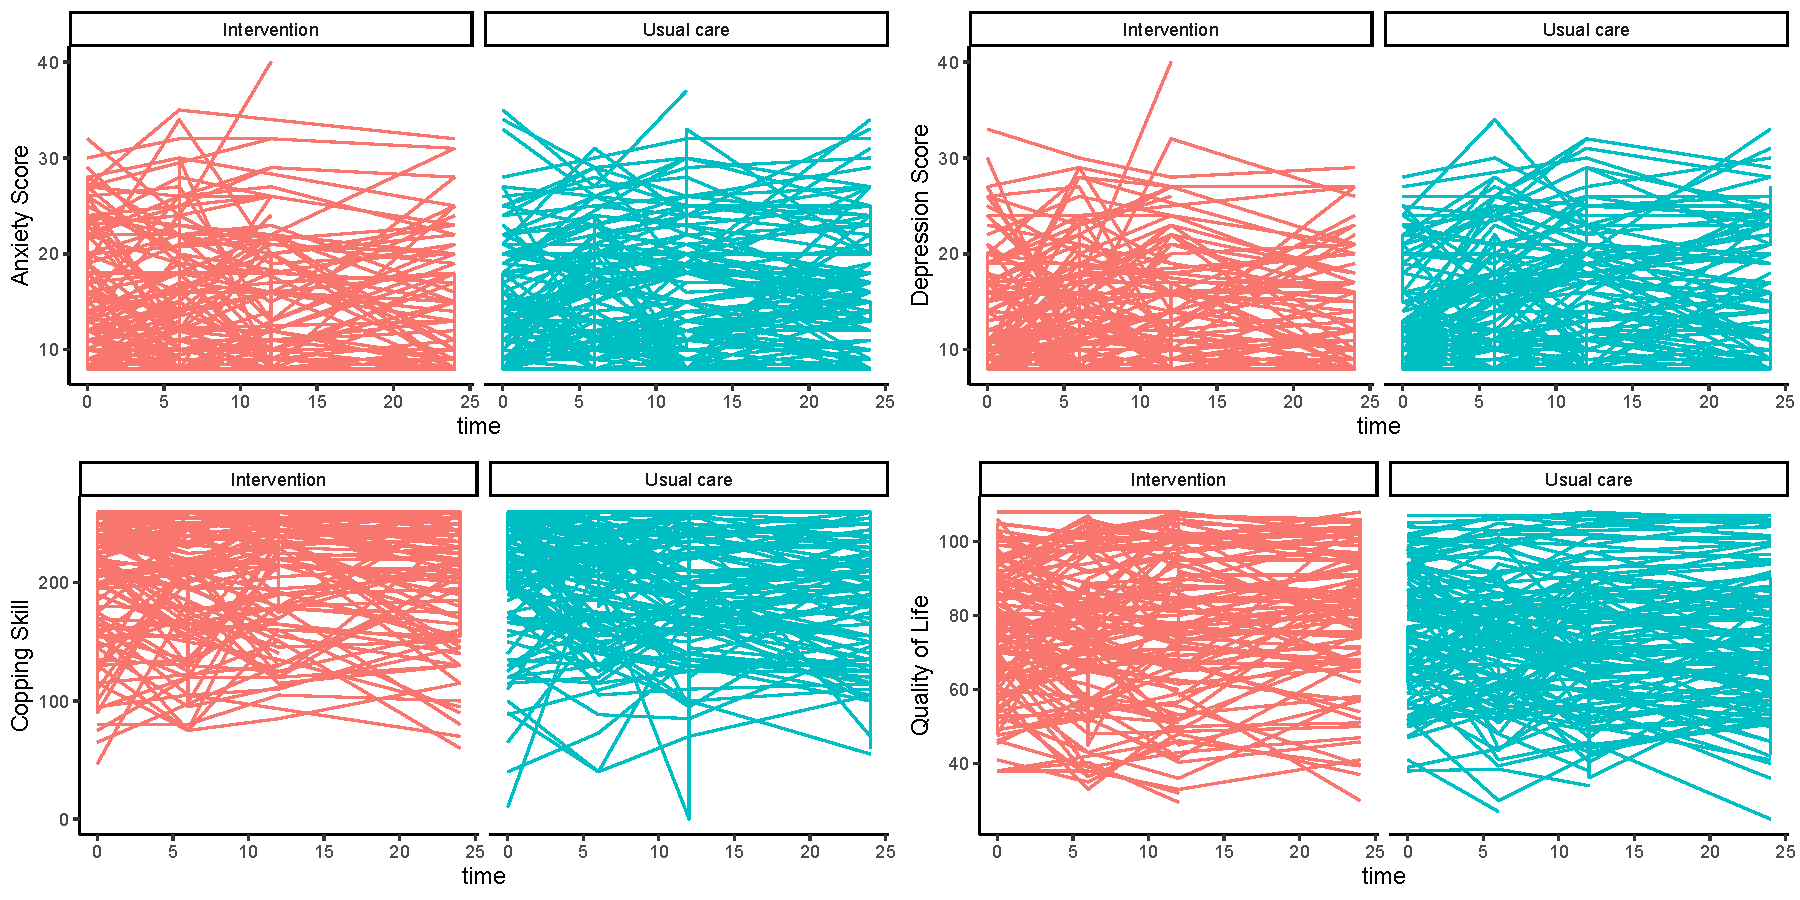
\includegraphics[width=0.8\linewidth]{homework2_solution_files/figure-latex/unnamed-chunk-1-1} \end{center}

\newpage

\hypertarget{question-2-glm-gzlm-and-lmm}{%
\section{Question 2 GLM, GzLM, and
LMM}\label{question-2-glm-gzlm-and-lmm}}

In a paragraph, explain the difference between a general linear model
(GLM; not a generalized linear model, which I denote with GzLM and which
will be discussed more later) and a linear mixed model (LMM).

\textcolor{blue}{Basically, a general linear model (GLM) is for independent (e.g., cross-sectional) data, and a linear mixed model (LMM) accounts for correlated data. The GLM is a special case of the LMM when there are no random effects and the error covariance matrix is simple ($\sigma^2 \pmb I$). Both modeling approaches are regression-type models, where we are trying to understand the relationship between an outcome and several.}

\newpage

\hypertarget{question-3-profiled-likelihood-restricted-likelihood-and-likelihood-functions}{%
\section{Question 3 Profiled likelihood, restricted likelihood, and
Likelihood
functions}\label{question-3-profiled-likelihood-restricted-likelihood-and-likelihood-functions}}

In a short paragraph, explain the difference between a profiled
likelihood and a restricted likelihood for a linear mixed model, and how
and why they are used. Which one is a re-expression of the standard
likelihood?

\textcolor{blue}{A profiled likelihood is a re-expression of the standard likelihood. The common profiled likelihood for a linear mixed model is expressed completely in terms of the covariance parameters. This is accomplished by maximizing the likelihood conditioned on the covariance parameters, and then solving for the fixed effects. This leads to an algebraic form for $\pmb {\hat \beta}$, expressed as a function of the covariance parameters. This form can then be substituted back in for $\pmb {\beta}$, so that the likelihood is completely expressed in terms of covariance parameters, but it is intrinsically the same likelihood. The restricted likelihood considers a linear form of the original $\pmb Y$ that eliminates the fixed effects completely, so it is a different likelihood. The purpose is to get unbiased (or at least less biased) estimators of covariance parameters. The difficulty is there is no true mechanism to estimate the fixed effect parameters with the restricted likelihood, so what is typically done is that the ML algebraic form for $\pmb {\hat \beta}$ is employed.}

\newpage

\hypertarget{question-4-variance-in-lmm}{%
\section{Question 4 Variance in LMM}\label{question-4-variance-in-lmm}}

Derive \(Var[\pmb {\hat \beta}]\) in a full-rank linear mixed model,
given the algebraic form of \(\pmb {\hat \beta}\) that is obtained via
ML estimation.

NOTE: there are two types of variance, model-based and empirical (or
sandwich estimator 🥪). The difference is whether the middle \(\pmb V\)
is determined via the model or using squared residual quantities; derive
\emph{the model-based form}. To answer this question, work with the
`complete data' form of \(\pmb {\hat \beta}\).

\textcolor{blue}{The ML estimator has form $\pmb {\hat \beta} = (\pmb X^t \pmb V^{-1}\pmb X)^-\pmb X^t\pmb V^{-1}\pmb Y$, which is a linear form of $\pmb Y$. Since we are dealing with a model with full rank $\pmb X$, then $\pmb {\hat \beta} = (\pmb X^t \pmb V^{-1} \pmb X)^{-1}\pmb X^t \pmb V^{-1}\pmb Y$. The linear form result says $Var[\pmb{AY}] = \pmb A Var[\pmb Y] \pmb A^t$; so let $\pmb A = (\pmb X^t \pmb V^{-1} \pmb X)^{-1} \pmb X^t \pmb V^{-1}$ and 

$$
\begin{aligned}
Var[\pmb {\hat \beta}] 
&= \pmb A Var[\pmb Y] \pmb A^t\\
&= \Big[(\pmb X^t \pmb V^{-1} \pmb X)^{-1} \pmb X^t \pmb V^{-1} \Big] Var[\pmb Y] \Big[(\pmb X^t \pmb V^{-1} \pmb X)^{-1} \pmb X^t \pmb V^{-1} \Big]^t\\
&= \Big[(\pmb X^t \pmb V^{-1} \pmb X)^{-1} \pmb X^t \pmb V^{-1} \Big] \pmb V \Big[(\pmb X^t \pmb V^{-1} \pmb X)^{-1} \pmb X^t \pmb V^{-1} \Big]^t\\
&= (\pmb X^t \pmb V^{-1} \pmb X)^{-1} \pmb X^t \pmb V^{-1} \pmb V (\pmb V^{-1})^{t} \pmb X  \Big[(\pmb X^t \pmb V^{-1} \pmb X)^{-1} \Big]^t\\
&= (\pmb X^t \pmb V^{-1} \pmb X)^{-1} \pmb X^t \pmb V^{-1} \pmb V \pmb V^{-1} \pmb X  \Big[(\pmb X^t \pmb V^{-1} \pmb X)^{-1} \Big]^t\\
&= (\pmb X^t \pmb V^{-1} \pmb X)^{-1} \pmb X^t \pmb V^{-1} \pmb X  (\pmb X^t \pmb V^{-1} \pmb X)^{-1} \\
&= (\pmb X^t \pmb V^{-1} \pmb X)^{-1} 
\end{aligned}
$$


Another good practice question is to derive $Var[\pmb {L\hat \beta}]$ for an estimable $\pmb {L\beta}$ , for a less-than-full-rank model.}

\end{document}
